\begin{spacing}{1}
  \chapter*{Abstract}
\end{spacing}
\begin{wrapfigure}{r}{0.3\textwidth}
  \begin{center}
    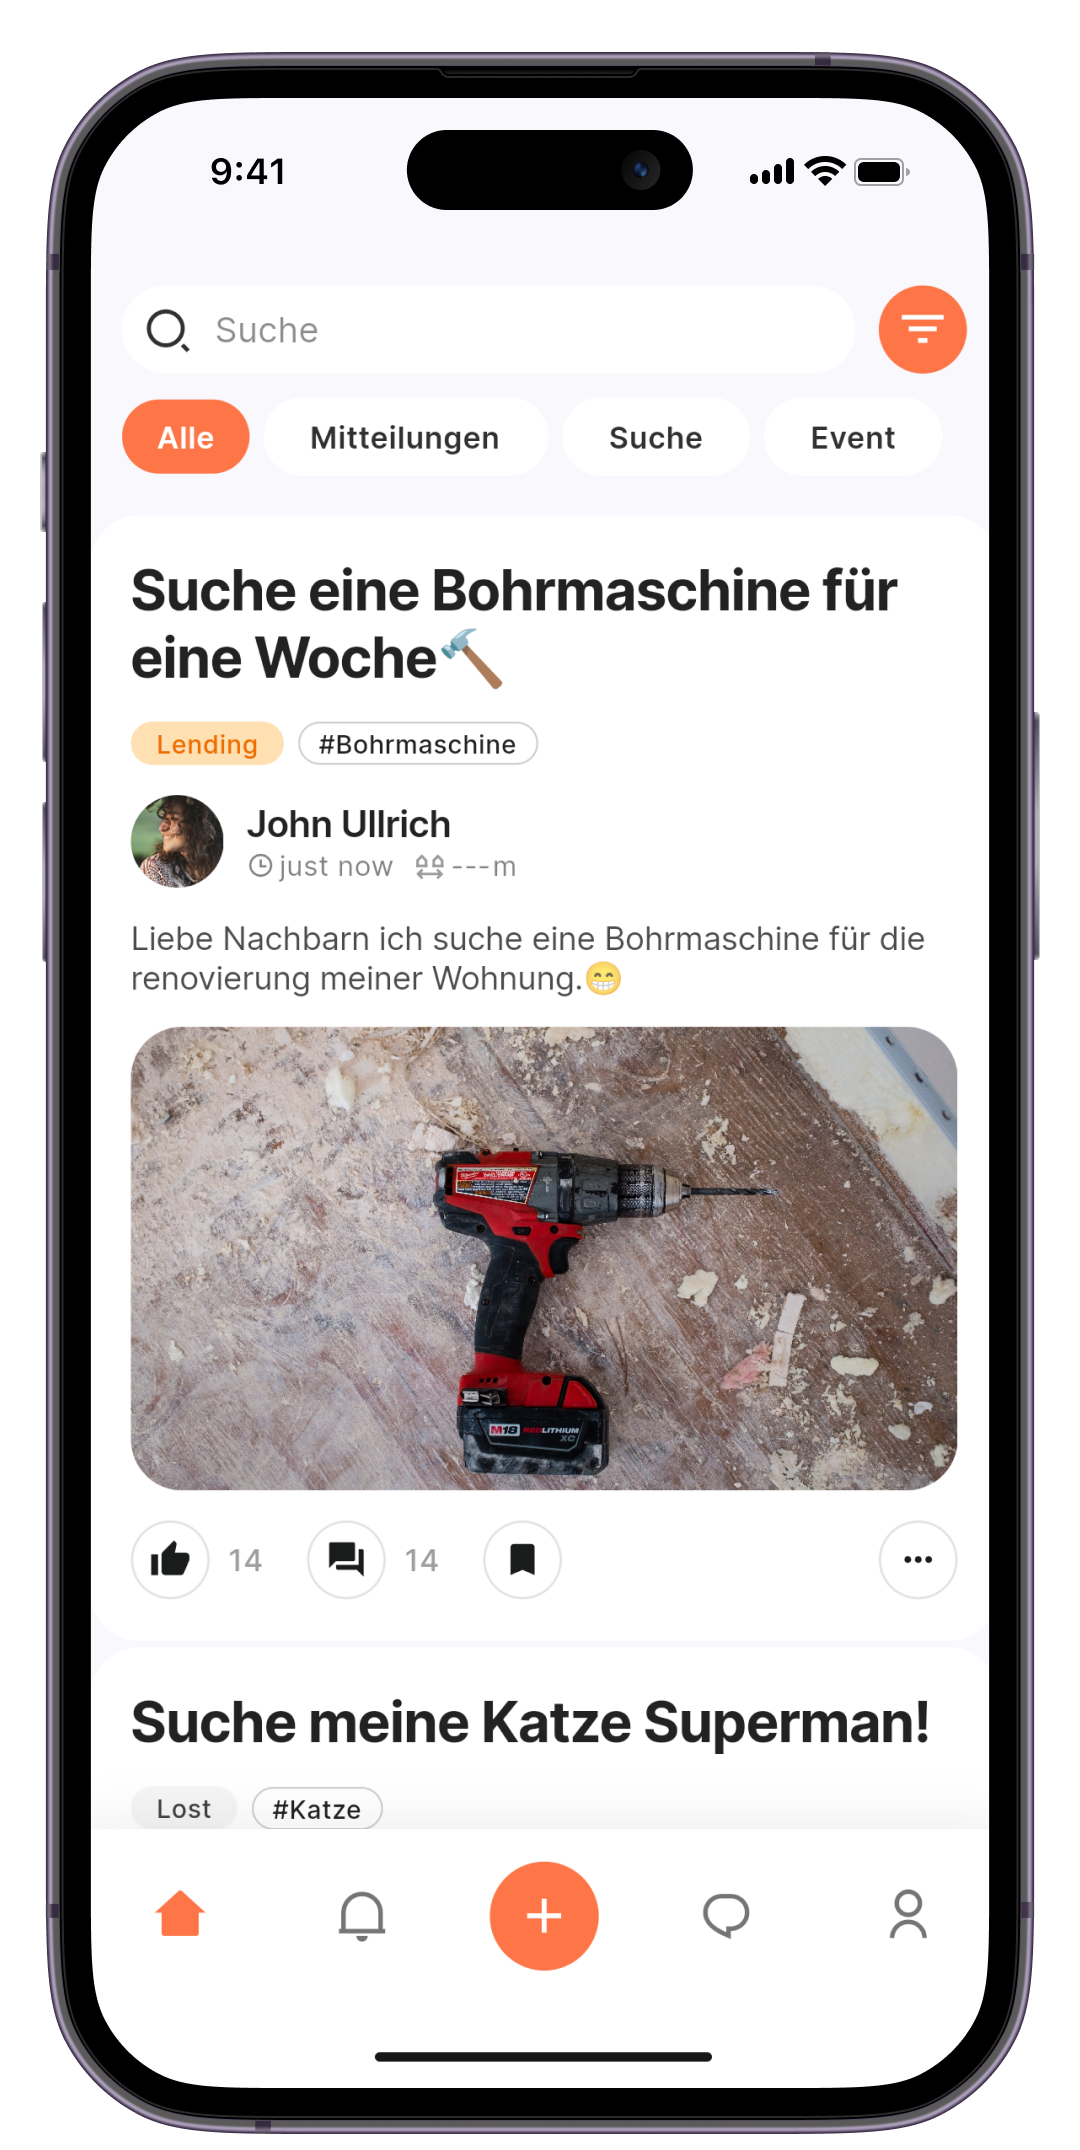
\includegraphics[width=0.3\textwidth]{pics/iphone.png}
  \end{center}
\end{wrapfigure}
The 2018 United Nations study \cite{un2018world} shows that the world population will increase to 9.7 billion people by 2050, with the majority of this increase taking place in urban areas. About 68\% of the world's population is expected to live in cities by 2050. These developments have far-reaching implications for the way we live and work together in cities.

The Nochba project works to strengthen communities and neighbourhoods in urban areas through various social networking initiatives and measures to promote social connections and cohesion between neighbours. With the increase in urban population by 2050, Project Nochba will play an important role in ensuring that neighbourhoods and communities in cities remain liveable and social isolation is reduced.

The app includes a translation function that helps overcome language barriers between community members. This allows users to search for and offer various forms of help to neighbours, such as shopping for elderly neighbours, helping with renovation work, fixing a flat tyre, looking for a lost pet or borrowing tools. The app also serves as a platform to warn neighbours of possible burglaries or other dangers. Users can verify their address when registering via location recognition or QR codes, with QR codes for communities being passed from phone to phone or published by the city or housing associations. Users can define the size of their community by setting a radius in which they can request or offer help via postings. Neighbours can then see and respond to these postings, and the app facilitates communication between those seeking help and those offering it.
\newpage
\begin{spacing}{1}
  \chapter*{Zusammenfassung}
\end{spacing}
\begin{wrapfigure}{r}{0.3\textwidth}
  \begin{center}
    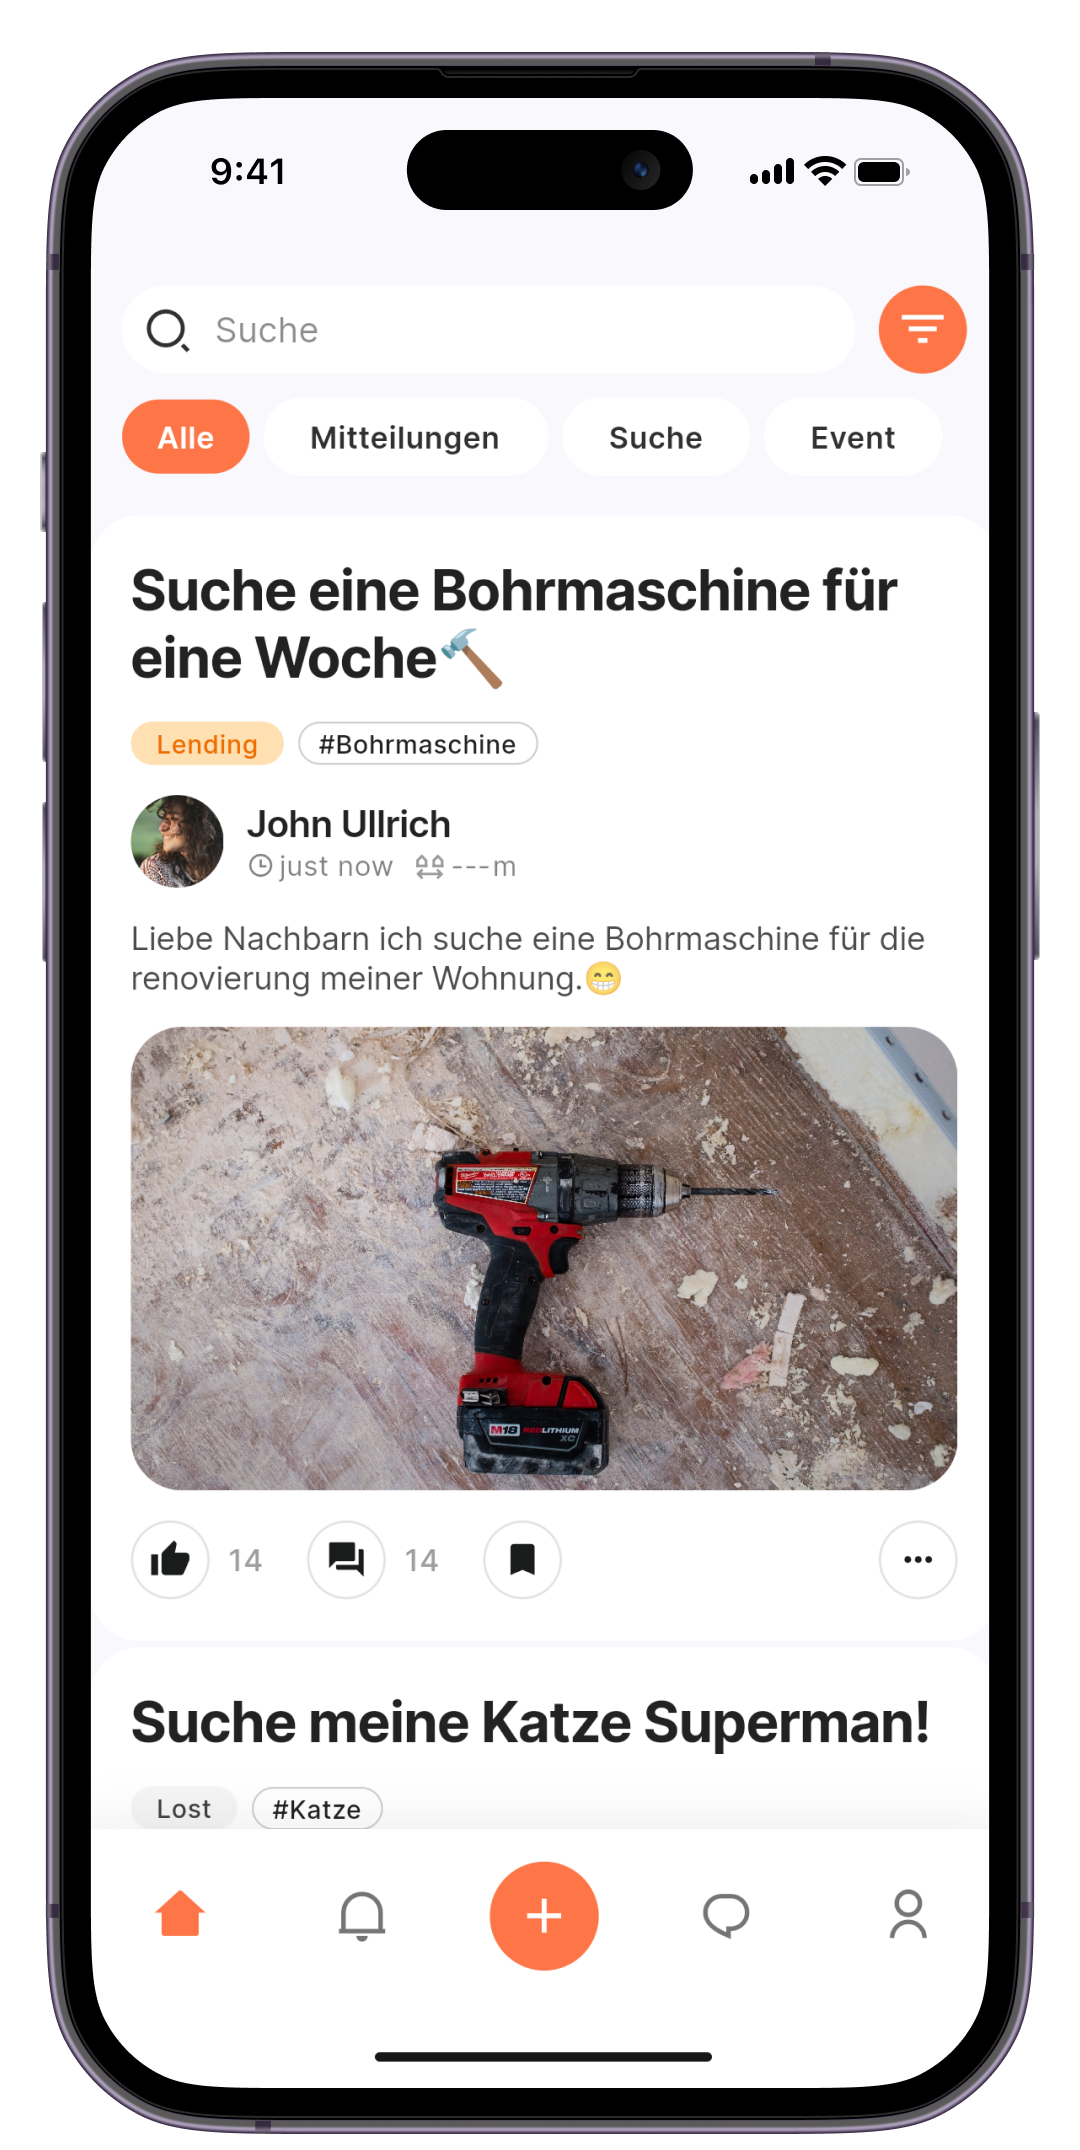
\includegraphics[width=0.3\textwidth]{pics/iphone.png}
  \end{center}
\end{wrapfigure}
Die Studie der Vereinten Nationen \cite{un2018world} aus dem Jahr 2018 zeigt, dass bis 2050 voraussichtlich ein Anstieg der Weltbevölkerung auf 9,7 Milliarden Menschen erwartet wird, wobei der größte Teil dieses Anstiegs in städtischen Gebieten stattfinden wird. Es wird erwartet, dass bis 2050 etwa 68\% der Weltbevölkerung in Städten leben werden. Diese Entwicklungen haben weitreichende Auswirkungen auf die Art und Weise, wie wir in Städten leben und zusammenarbeiten.

Das Projekt Nochba setzt sich dafür ein, die Gemeinschaft und Nachbarschaften in städtischen Gebieten zu stärken, indem es verschiedene Initiativen und Maßnahmen ergreift, um soziale Verbindungen und Zusammenhalt zwischen den Nachbarn zu fördern. Angesichts des Anstiegs der städtischen Bevölkerung bis 2050 wird das Projekt Nochba eine wichtige Rolle dabei spielen, sicherzustellen, dass die Nachbarschaften und Gemeinschaften in Städten weiterhin lebenswert bleiben und dass soziale Isolation reduziert wird.

Die App enthält eine Übersetzungsfunktion, die hilft, Sprachbarrieren zwischen den Mitgliedern der Gemeinschaft zu überwinden. So können die Nutzer unterschiedliche Formen der Nachbarschaftshilfe suchen und anbieten, beispielsweise für ältere Nachbarn einkaufen, bei Renovierungsarbeiten helfen, eine Reifenpanne beheben, ein entlaufenes Haushaustier suchen oder Werkzeuge ausleihen. Die App dient auch als Plattform, um Nachbarn vor möglichen Einbrüchen oder anderen Gefahren zu warnen. Die Nutzer können ihre Adresse während der Registrierung über die Standorterkennung oder QR-Codes verifizieren, wobei QR-Codes für Gemeinschaften von Telefon zu Telefon weitergegeben oder von der Stadt oder Wohnungsbaugenossenschaften veröffentlicht werden. Die Nutzer können die Größe ihrer Community definieren, indem sie einen Radius festlegen, innerhalb dessen sie über Postings Hilfe anfordern oder anbieten können. Die Nachbarn können dann diese Beiträge sehen und darauf antworten, und die App erleichtert die Kommunikation zwischen Hilfesuchenden und Helfern.

